\chapter{Kimia Lingkungan dan Toksikologi}\label{ch:b3:environmental-toxicology}

Setiap akhir musim panas, satelit memotret pusaran hijau yang menyebar di danau-danau
besar: ledakan alga yang disuburkan oleh fosfat dan nitrat yang mengalir dari ladang dan
keluar dari kota. Ketika alga itu mati dan tenggelam, pembusukannya menghabiskan oksigen di
air dalam, dan ikan-ikan mati. Kimia menjelaskan setiap mata rantai itu, dan
banyak rantai lainnya: mengapa sebagian gas menghangatkan planet dan yang lain tidak, mengapa hujan
bersifat asam bahkan di udara yang bersih, ke mana sebuah pestisida pergi setelah disemprotkan, dan
berapa banyak suatu zat yang diperlukan untuk menimbulkan bahaya. Bab ini menerapkan kesetimbangan,
kinetika, dan spektroskopi pada atmosfer, perairan alami, dan tanah, menelusuri
polutan di antara ketiganya, dan ditutup dengan angka-angka yang menjadi dasar penilaian
risiko.

\begin{recall}
Jilid Tahun 1 mencakup kesetimbangan asam--basa, pengendapan, dan
kompleksasi, diagram potensial--pH, koefisien partisi, waktu paruh, bahaya,
risiko, dan sistem GHS; jilid sekolah membahas \omterm{def:b3:environmental-toxicology:greenhouse}{gas rumah kaca}; Jilid Tahun 2 membahas
hukum Henry, kekuatan ion, statistika, spektrometri massa, dan spektrometri
atom. \Cref{ch:b3:photochemistry} membahas fotokimia atmosfer,
\cref{ch:b3:group-theory-applied} dan \cref{ch:b3:rovibrational-spectroscopy}
keaktifan inframerah, dan \cref{ch:b3:surfaces-catalysis} \omterm{def:b3:surfaces-catalysis:adsorption}{adsorpsi}.
\end{recall}

\begin{omfigure}
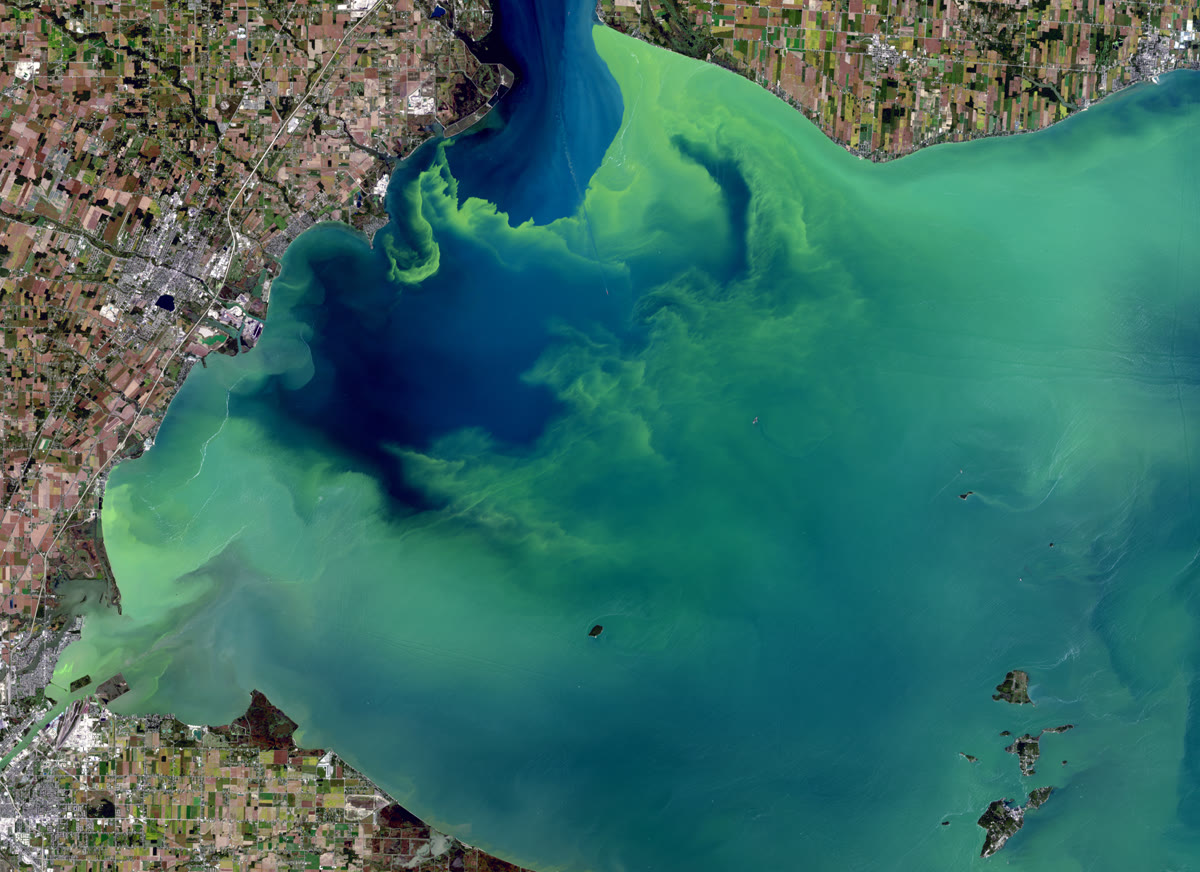
\includegraphics[width=0.62\linewidth]{images/book4/algal-bloom.jpg}

{\small Ledakan alga di sebuah danau besar, yang dilihat oleh satelit pengamat Bumi pada
akhir September: pusaran-pusaran hijau itu adalah populasi padat alga mikroskopis
yang disuburkan oleh nutrien dari lahan pertanian di sekitarnya. Gambar: USGS dan NASA, domain publik.}
\end{omfigure}

\section{Atmosfer}

\begin{definition}[Gas rumah kaca]\label{def:b3:environmental-toxicology:greenhouse}
Yang disebut \emph{gas rumah kaca}\index{gas rumah kaca} adalah gas yang menyerap dan memancarkan radiasi
inframerah pada panjang gelombang radiasi yang dipancarkan permukaan Bumi, sehingga
menghangatkan atmosfer bawah. Yang disebut \emph{potensi pemanasan
global}\index{potensi pemanasan global} (GWP) sebuah gas dalam suatu cakrawala waktu,
biasanya 100 tahun, adalah energi yang diperangkapnya setelah emisi satu kilogram gas itu,
relatif terhadap satu kilogram karbon dioksida.
\end{definition}

Sebuah molekul menyerap radiasi inframerah hanya melalui vibrasi yang mengubah
momen dipolnya (\cref{ch:b3:group-theory-applied}). Dinitrogen dan dioksigen,
yaitu molekul diatomik homonuklir, tidak memiliki vibrasi semacam itu dan transparan; argon sama sekali tidak memiliki
vibrasi. Karbon dioksida, yang linear dan nonpolar, memiliki modus tekuk yang aktif inframerah
di dekat \qty{15}{\micro\metre}, di tengah-tengah emisi Bumi; air, metana,
dan dinitrogen oksida menyerap pada banyak panjang gelombang.

% ledger: atm:CO2.2025, atm:CH4.2025, atm:N2O.2025, gwp:CH4.fossil, gwp:CH4.nonfossil, gwp:N2O, life:CH4, life:N2O
Pada 2025, fraksi mol rata-rata global adalah \qty{425.6}{ppm} karbon dioksida, \qty{1936}{ppb}
metana, dan \qty{338.9}{ppb} dinitrogen oksida. Metana, yang disingkirkan oleh radikal hidroksil dengan
umur sekitar 12 tahun, memiliki GWP-100 sebesar 27 sampai 30; dinitrogen oksida, yang hanya dimusnahkan di
stratosfer dengan umur sekitar 109 tahun, memiliki nilai 273. Karbon dioksida tidak memiliki
satu umur tunggal: sebagian emisinya tetap berada di udara selama berabad-abad.

\begin{definition}[Polutan udara]\label{def:b3:environmental-toxicology:pollutants}
Yang disebut \emph{materi partikulat}\index{materi partikulat} adalah partikel padat dan cair
yang melayang di udara, yang digolongkan menurut diameter aerodinamisnya (partikel halus
yang lebih kecil daripada \qty{2.5}{\micro\metre} mencapai bagian dalam paru-paru). Yang disebut \emph{hujan
asam}\index{hujan asam} adalah hujan yang dibuat lebih asam daripada hujan bersih oleh asam sulfat dan
asam nitrat yang terbentuk dari belerang dioksida dan nitrogen oksida.
\end{definition}

\begin{proposition}[pH hujan bersih]\label{prop:b3:environmental-toxicology:rain-ph}
Hujan yang berada dalam kesetimbangan dengan karbon dioksida udara masa kini, dan tidak dengan zat
lain, memiliki pH sekitar 5.6.
\end{proposition}

\begin{proof}
% ledger: henry:CO2, pka4:H2CO3.1, pkw4:25C, const:atm
Hukum Henry memberikan $[\ce{CO2(aq)}] = K_Hp(\ce{CO2}) = \qty{3.4e-7}{mol.L^{-1}.Pa^{-1}} \times (425.6 \times 10^{-6} \times \qty{101325}{Pa}) = \qty{1.47e-5}{mol/L}$.
Neraca muatannya adalah $[\ce{H+}] = [\ce{HCO3-}] + 2[\ce{CO3^2-}] + [\ce{OH-}] \approx K_{a1}[\ce{CO2(aq)}]/[\ce{H+}] + K_w/[\ce{H+}]$, sehingga
$[\ce{H+}]^2 = K_{a1}[\ce{CO2(aq)}] + K_w = 10^{-6.35} \times \num{1.47e-5} + 10^{-14} = \num{6.6e-12}$: $[\ce{H+}] = \qty{2.6e-6}{mol/L}$, pH 5.6.
\end{proof}

Belerang dioksida dari pembakaran bahan bakar yang mengandung belerang dan nitrogen oksida dari
pembakaran bersuhu tinggi dioksidasi di udara, oleh radikal hidroksil dan di dalam tetesan
awan, menjadi asam sulfat dan asam nitrat, yang menurunkan pH hujan sampai 4 dan di bawahnya.
Penyingkiran belerang dari bahan bakar dan nitrogen oksida dari gas buang (konverter
katalitik, injeksi amonia di pembangkit listrik) telah sebagian besar menyelesaikan masalah itu
di tempat-tempat penerapannya. Ozon di dekat permukaan tanah, yang terbentuk ketika sinar matahari bekerja pada
nitrogen oksida dan senyawa organik atsiri (\cref{ch:b3:photochemistry}), dan
partikel halus tetap menjadi polutan udara utama bagi kesehatan.

\section{Perairan alami}

\begin{omfigure}
\begin{tikzpicture}
\begin{axis}[name=a, width=0.48\linewidth, height=5.4cm, xmin=4, xmax=13, ymin=0, ymax=1.02,
  axis lines=left, xlabel={pH}, ylabel={fraksi karbon terlarut},
  tick label style={font=\scriptsize}, label style={font=\small}]
\addplot[color=omDef, thick] table[x=pH, y=a0] {figdata/out/bachelor-3-carbonate-system.dat};
\addplot[color=omMeth, thick] table[x=pH, y=a1] {figdata/out/bachelor-3-carbonate-system.dat};
\addplot[color=omThm, thick] table[x=pH, y=a2] {figdata/out/bachelor-3-carbonate-system.dat};
\node[font=\scriptsize, omDef] at (axis cs:4.9,0.85) {$\ce{CO2(aq)}$};
\node[font=\scriptsize, omMeth] at (axis cs:8.3,0.88) {$\ce{HCO3-}$};
\node[font=\scriptsize, omThm] at (axis cs:12.1,0.85) {$\ce{CO3^2-}$};
\draw[black!30, dashed] (axis cs:6.35,0) -- (axis cs:6.35,0.5) (axis cs:10.33,0) -- (axis cs:10.33,0.5);
\end{axis}
\begin{axis}[at={(a.east)}, anchor=west, xshift=1.4cm, width=0.48\linewidth, height=5.4cm,
  xmin=0, xmax=2000, ymin=5.2, ymax=6.2, axis lines=left,
  xlabel={$\ce{CO2}$ di udara / ppm}, ylabel={pH hujan},
  tick label style={font=\scriptsize}, label style={font=\small},
  scaled x ticks=false, xticklabel style={/pgf/number format/1000 sep={}}]
\addplot[color=omDef, thick] table[x=ppm, y=pH] {figdata/out/bachelor-3-carbonate-system-b.dat};
\draw[black!35, dashed] (axis cs:425.6,5.2) -- (axis cs:425.6,5.59);
\node[font=\scriptsize, anchor=west] at (axis cs:470,5.63) {kini: 5.6};
\end{axis}
\end{tikzpicture}

{\small Kiri: distribusi karbon anorganik terlarut di antara ketiga bentuknya
terhadap pH pada \qty{25}{\celsius}, yang bersilangan pada $\mathrm pK_{a1} = 6.35$ dan $\mathrm pK_{a2} = 10.33$. Kanan: pH hujan yang berada dalam
kesetimbangan dengan karbon dioksida saja, terhadap fraksi molnya di udara.}
\end{omfigure}

\begin{proposition}[Fraksi karbonat]\label{prop:b3:environmental-toxicology:carbonate-fractions}
Dengan $C_T$ karbon anorganik terlarut total,
$[\ce{CO2(aq)}] = C_Th^2/D$, $[\ce{HCO3-}] = C_TK_{a1}h/D$, $[\ce{CO3^2-}] = C_TK_{a1}K_{a2}/D$, dengan $h = [\ce{H+}]$ dan $D = h^2 + K_{a1}h + K_{a1}K_{a2}$.
\end{proposition}

\begin{proof}
Dari kedua tetapan keasaman,
\[
  [\ce{HCO3-}] = \frac{K_{a1}[\ce{CO2(aq)}]}{h}, \qquad [\ce{CO3^2-}] = \frac{K_{a2}[\ce{HCO3-}]}{h} = \frac{K_{a1}K_{a2}[\ce{CO2(aq)}]}{h^2}.
\]
Jumlah ketiganya adalah $C_T = [\ce{CO2(aq)}]\,D/h^2$; membagi setiap bentuk dengan $C_T$ memberikan fraksi-fraksinya.
\end{proof}

\begin{definition}[Alkalinitas]\label{def:b3:environmental-toxicology:alkalinity}
Yang disebut \emph{alkalinitas}\index{alkalinitas} sebuah air adalah kapasitasnya untuk menetralkan
asam kuat, yang diukur dengan titrasi sampai titik akhir asam karbonat (sekitar pH
4.5) dan dinyatakan dalam mol $\ce{H+}$ per liter.
\end{definition}

\begin{proposition}[Alkalinitas karbonat]\label{prop:b3:environmental-toxicology:alkalinity}
Dalam air yang basa-basanya berupa spesies karbonat dan hidroksida,
$\mathrm{Alk} = [\ce{HCO3-}] + 2[\ce{CO3^2-}] + [\ce{OH-}] - [\ce{H+}]$; \omterm{def:b3:environmental-toxicology:alkalinity}{alkalinitas} itu sama dengan kelebihan muatan kation basa kuat
atas muatan anion asam kuat, dan tidak berubah ketika karbon dioksida
dipertukarkan dengan udara.
\end{proposition}

\begin{proof}
Titrasi sampai titik akhir asam karbonat mengubah setiap $\ce{HCO3-}$ menjadi $\ce{CO2}$ (masing-masing satu $\ce{H+}$),
setiap $\ce{CO3^2-}$ menjadi $\ce{CO2}$ (dua), dan setiap $\ce{OH-}$ menjadi air (satu), sedangkan $\ce{H+}$ bebas yang sudah ada
dihitung sebagai pengurang: itulah jumlah yang dinyatakan. Neraca muatan air itu, dengan
$\ce{Na+}$, $\ce{Ca^2+}$\dots{} dan $\ce{Cl-}$, $\ce{SO4^2-}$\dots, dapat disusun ulang menjadi jumlah yang sama, yang setara dengan $\sum z_i c_i$(kation) $-$ $\sum z_jc_j$(anion)
elektrolit-elektrolit kuat. Menambahkan atau menyingkirkan $\ce{CO2}$ tidak mengubah satu pun ion itu.
\end{proof}

\begin{definition}[Pengasaman laut]\label{def:b3:environmental-toxicology:acidification}
Yang disebut \emph{pengasaman laut}\index{pengasaman laut} adalah penurunan
pH air laut ketika air itu menyerap karbon dioksida dari udara. Yang disebut \emph{keadaan
kejenuhan}\index{keadaan kejenuhan} sebuah mineral karbonat adalah
$\Omega = [\ce{Ca^2+}][\ce{CO3^2-}]/K_{sp}$: di atas 1 mineral itu dapat terbentuk, di bawah 1 mineral itu cenderung larut.
\end{definition}

Karbon dioksida terlarut mengubah ion karbonat menjadi hidrogenkarbonat, $\ce{CO2 + CO3^2- + H2O -> 2HCO3-}$,
sehingga menurunkan pH dan $\Omega$: cangkang dan kerangka karang menjadi lebih sulit dibangun. (Dalam
air laut, tetapan-tetapannya adalah tetapan semu, yang diukur dalam medium garam, dan
berbeda dari nilai-nilai air tawar pada bab ini.)

\begin{definition}[Kesadahan air]\label{def:b3:environmental-toxicology:hardness}
Yang disebut \emph{kesadahan}\index{kesadahan air} sebuah air adalah konsentrasi total
ion kalsium dan magnesiumnya, yang sering dinyatakan sebagai massa kalsium karbonat
yang akan mengandung jumlah mol yang sama, dalam mg/L.
\end{definition}

\begin{definition}[Kebutuhan oksigen]\label{def:b3:environmental-toxicology:oxygen-demand}
Yang disebut \emph{kebutuhan oksigen biokimia}\index{kebutuhan oksigen biokimia} (BOD) sebuah
air adalah massa dioksigen yang dikonsumsi per liter oleh mikroorganisme yang mengoksidasi
bahan organiknya dalam gelap, selama waktu tertentu (lima hari pada \qty{20}{\celsius} untuk $\mathrm{BOD_5}$). Yang disebut
\emph{kebutuhan oksigen kimia}\index{kebutuhan oksigen kimia} (COD) air itu adalah massa
dioksigen yang setara dengan dikromat yang dikonsumsi untuk mengoksidasi bahan organiknya
secara kimia.
\end{definition}

\begin{proposition}[Kurva BOD]\label{prop:b3:environmental-toxicology:bod}
Jika bahan organik yang dapat terbiodegradasi dikonsumsi dengan kinetika orde satu dengan tetapan
laju $k$, oksigen yang terpakai setelah waktu $t$ adalah $\mathrm{BOD}_t = L_0(1 - \eu^{-kt})$, dengan $L_0$ BOD akhir.
\end{proposition}

\begin{proof}
Kebutuhan yang tersisa $L$ mematuhi $\dd L/\dd t = -kL$, sehingga $L = L_0\eu^{-kt}$; oksigen yang terpakai adalah bagian yang telah hilang,
$L_0 - L$.
\end{proof}

\begin{omfigure}
\begin{tikzpicture}
\begin{axis}[name=a, width=0.48\linewidth, height=5.2cm, xmin=0, xmax=30, ymin=0, ymax=270,
  axis lines=left, xlabel={waktu / hari}, ylabel={BOD / \unit{mg.L^{-1}}},
  tick label style={font=\scriptsize}, label style={font=\small}]
\addplot[color=omDef, thick] table[x=t, y=bod] {figdata/out/bachelor-3-bod.dat};
\draw[black!35, dashed] (axis cs:0,250) -- (axis cs:30,250);
\draw[black!35, dashed] (axis cs:5,0) -- (axis cs:5,170.8);
\node[font=\scriptsize, anchor=west] at (axis cs:5.6,140) {$\mathrm{BOD_5}$};
\node[font=\scriptsize, anchor=north east] at (axis cs:30,246) {$L_0$};
\end{axis}
\begin{axis}[at={(a.east)}, anchor=west, xshift=1.4cm, width=0.48\linewidth, height=5.2cm,
  xmin=0, xmax=15, ymin=0, ymax=10, axis lines=left,
  xlabel={waktu ke hilir / hari}, ylabel={$\ce{O2}$ terlarut / \unit{mg.L^{-1}}},
  tick label style={font=\scriptsize}, label style={font=\small}]
\addplot[color=omThm, thick] table[x=t, y=O2] {figdata/out/bachelor-3-bod-b.dat};
\draw[black!35, dashed] (axis cs:0,9.1) -- (axis cs:15,9.1);
\node[font=\scriptsize, anchor=south east] at (axis cs:15,9.1) {kejenuhan};
\node[font=\scriptsize, anchor=north] at (axis cs:2.4,6.3) {titik kritis};
\end{axis}
\end{tikzpicture}

{\small Kiri: BOD limbah model, $L_0 = \qty{250}{mg/L}$ dan $k = \qty{0.23}{d^{-1}}$: sekitar dua pertiga
kebutuhan itu terpakai dalam lima hari. Kanan: penurunan oksigen di sungai di bawah sebuah saluran keluar
(model Streeter--Phelps): penguraian beban organik mula-mula mengonsumsi oksigen lebih cepat daripada
yang dapat dipulihkan oleh udara, sampai defisitnya memuncak setelah sekitar 2.4 hari.}
\end{omfigure}

\begin{method}[Menentukan COD]\label{met:b3:environmental-toxicology:cod}
\begin{enumerate}
  \item Refluks volume sampel yang terukur dengan kalium dikromat berlebih yang diketahui
        jumlahnya dalam asam sulfat, dengan perak sulfat sebagai katalis dan
        raksa(II) sulfat untuk mengikat klorida.
  \item Titrasi dikromat yang tersisa dengan besi(II) memakai feroin, dan jalankan
        blangko dengan air murni.
  \item Dikromat yang terpakai, yang dikonversi menjadi massa $\ce{O2}$ yang setara (satu
        $\ce{Cr2O7^2-}$ menerima enam elektron, seperti yang akan dilakukan 1.5 $\ce{O2}$), dibagi dengan volume sampel, adalah
        COD dalam mg/L.
\end{enumerate}
\end{method}

\begin{definition}[Eutrofikasi]\label{def:b3:environmental-toxicology:eutrophication}
Yang disebut \emph{eutrofikasi}\index{eutrofikasi} adalah pengayaan badan air
dengan nutrien, terutama fosfor dan nitrogen, yang menyebabkan pertumbuhan berlebihan
alga dan tumbuhan, lalu penipisan oksigen ketika alga dan tumbuhan itu membusuk.
\end{definition}

\begin{omfigure}
\begin{tikzpicture}[font=\scriptsize, >=Stealth,
  box/.style={draw, rounded corners, align=center, fill=omMeth!10, inner sep=3pt, minimum height=8mm}]
  \node[box] (f) at (-3.9,1.2) {ladang: pupuk,\\ pupuk kandang};
  \node[box] (t) at (-3.9,-0.4) {kota: limbah,\\ deterjen};
  \node[box] (a) at (0,2.1) {atmosfer:\\ deposisi (N)};
  \node[box, fill=omDef!12, minimum width=3.2cm, minimum height=1.7cm] (l) at (0.6,0.4) {air danau:\\ alga tumbuh};
  \node[box, fill=black!8] (s) at (0.6,-1.6) {sedimen: P tersimpan,\\ dilepaskan saat anoksik};
  \node[box] (o) at (4.0,0.4) {aliran keluar};
  \draw[->, thick] (f) -- node[above, sloped, pos=0.5] {limpasan} (l);
  \draw[->, thick] (t) -- node[below, sloped] {N, P} (l);
  \draw[->, thick] (a) -- (l);
  \draw[->, thick] (l) -- node[left] {alga mati} (s);
  \draw[->, thick, dashed] (s.east) to[bend right=30] node[right] {P} (l.south east);
  \draw[->, thick] (l) -- (o);
\end{tikzpicture}

{\small Aliran nutrien ke dalam dan di dalam danau. Fosfor, yang sering menjadi nutrien
pembatas di air tawar, menumpuk di sedimen dan kembali ke air
ketika dasar danau kehilangan oksigennya, dan hal itu dapat mempertahankan ledakan alga bertahun-tahun setelah
masukannya dihentikan.}
\end{omfigure}

Alga menyerap karbon, nitrogen, dan fosfor dalam perbandingan yang kira-kira tetap;
nutrien mana pun yang kurang dibandingkan dengan kebutuhan itu membatasi pertumbuhannya. Di
sebagian besar danau, nutrien itu adalah fosfor, dan itulah sebabnya fosfat disingkirkan dari
deterjen dan dari limbah yang diolah; di banyak laut pesisir, nutrien itu adalah nitrogen.

\begin{definition}[Spesiasi]\label{def:b3:environmental-toxicology:speciation}
Yang disebut \emph{spesiasi kimia}\index{spesiasi kimia} sebuah unsur dalam sebuah
sampel adalah distribusi jumlahnya di antara bentuk-bentuk kimianya: bilangan
oksidasi, kompleks, senyawa organologam, spesies bebas dan terikat.
\end{definition}

Toksisitas bergantung pada spesiasi. Raksa anorganik yang dilepaskan ke dalam air
dimetilasi oleh bakteri di sedimen menjadi metilraksa, yang menembus membran,
mengikat belerang protein, dan memekat sepanjang rantai makanan; arsenik jauh lebih
beracun sebagai arsenit, As(III), daripada sebagai arsenat, As(V), dan jauh kurang beracun dalam bentuk-bentuk
organik yang terdapat dalam makanan laut. Konsentrasi total saja tidak banyak berarti.

\begin{method}[Spesiasi logam dalam air]\label{met:b3:environmental-toxicology:speciation}
\begin{enumerate}
  \item Daftarlah ligan-ligan yang ada (hidroksida, karbonat, klorida, sulfat, bahan
        organik) beserta konsentrasinya dan pH-nya.
  \item Tuliskan tetapan-tetapan kompleksasi dan neraca massa logam itu, seperti pada
        Jilid Tahun 1.
  \item Selesaikan untuk ion logam bebas, lalu setiap kompleks; gambarlah fraksinya terhadap
        pH atau terhadap konsentrasi ligan.
  \item Bandingkan bentuk yang beracun atau yang tersedia secara hayati (sering ion bebas) dengan totalnya.
\end{enumerate}
\end{method}

\section{Tanah dan sedimen}

\begin{definition}[Sorpsi dalam tanah]\label{def:b3:environmental-toxicology:soil}
Yang disebut \emph{kapasitas tukar kation}\index{kapasitas tukar kation} sebuah tanah adalah
jumlah kation yang dapat dipertukarkan yang dapat ditahannya per satuan massa, pada lempung dan bahan
organik. Yang disebut \emph{koefisien distribusi tanah--air}\index{koefisien distribusi tanah--air}
$K_d$ adalah rasio konsentrasi suatu zat yang
tersorpsi pada tanah (per kilogram) terhadap konsentrasinya dalam air pori (per
liter); \emph{koefisien partisi karbon organik}\index{koefisien partisi karbon organik}
adalah $K_{oc} = K_d/f_{oc}$, dengan $f_{oc}$ fraksi massa karbon organik.
\end{definition}

Senyawa organik netral tersorpsi terutama pada bahan organik tanah, sehingga $K_{oc}$ jauh
kurang bervariasi dari satu tanah ke tanah lain daripada $K_d$. Senyawa dengan $K_d$ kecil bergerak bersama air
dan dapat mencapai air tanah (pelindian); senyawa dengan $K_d$ besar tetap di dekat permukaan,
terikat pada partikel yang dapat terbawa erosi ke sungai dan danau.

\section{Nasib polutan}

\begin{definition}[Koefisien partisi oktanol--air]\label{def:b3:environmental-toxicology:kow}
Yang disebut \emph{koefisien partisi oktanol--air}\index{koefisien partisi oktanol--air}
$K_{ow}$ suatu zat adalah rasio konsentrasi kesetimbangannya dalam
oktan-1-ol dan dalam air; koefisien itu mengukur afinitas zat itu terhadap jaringan lemak dan bahan
organik.
\end{definition}

% ledger: logkow:DDT, logkow:benzene, logkow:atrazine, logkow:PCB153
Benzena memiliki $\log K_{ow} = 2.13$, herbisida atrazina 2.61, sebuah PCB berklor enam 6.67, dan
DDT 6.91: dua yang terakhir larut dalam lemak puluhan juta kali lebih baik daripada dalam
air.

\begin{definition}[Bioakumulasi]\label{def:b3:environmental-toxicology:bio}
Yang disebut \emph{faktor biokonsentrasi}\index{faktor biokonsentrasi} (BCF) adalah
rasio konsentrasi dalam sebuah organisme terhadap konsentrasi dalam air di sekelilingnya pada
keadaan tunak, dengan penyerapan dari air saja. Yang disebut \emph{bioakumulasi}\index{bioakumulasi}
adalah penumpukan dalam organisme melalui semua jalur, termasuk makanan; sedangkan
\emph{biomagnifikasi}\index{biomagnifikasi} adalah kenaikan
konsentrasi dari mangsa ke pemangsa sepanjang rantai makanan.
\end{definition}

\begin{proposition}[BCF dan $K_{ow}$]\label{prop:b3:environmental-toxicology:bcf-kow}
Untuk zat organik netral yang tidak dimetabolisme, $\log\mathrm{BCF}$ pada ikan
kira-kira merupakan fungsi linear $\log K_{ow}$, dengan kemiringan mendekati 1, sampai $\log K_{ow}$ di dekat 6;
di atasnya, penyerapan melambat dan hubungan itu mendatar (regresi empiris).
\admitted
\end{proposition}

\begin{definition}[Polutan organik persisten]\label{def:b3:environmental-toxicology:pop}
Yang disebut \emph{polutan organik persisten}\index{polutan organik persisten} adalah
zat organik yang tahan terhadap penguraian, terbioakumulasi, beracun, dan
terangkut jauh dari sumbernya, seperti DDT, PCB, dan dioksin.
\end{definition}

\begin{proposition}[Distribusi kesetimbangan antarkompartemen]\label{prop:b3:environmental-toxicology:level-one}
Massa $M$ suatu zat yang terdistribusi pada kesetimbangan (model ``tingkat I'') di antara air
(volume $V_w$), udara ($V_a$), padatan sedimen ($m_s$), dan ikan ($m_f$) memiliki konsentrasi air
$C_w = M/(V_w + K_{aw}V_a + K_{sw}m_s + K_{fw}m_f)$, dengan $K$ koefisien-koefisien partisi relatif terhadap
air; massa dalam setiap kompartemen adalah sukunya kali $C_w$.
\end{proposition}

\begin{proof}
Pada kesetimbangan $C_a = K_{aw}C_w$, $C_s = K_{sw}C_w$ (per kilogram), $C_f = K_{fw}C_w$. Neraca massanya adalah
$M = C_wV_w + C_aV_a + C_sm_s + C_fm_f = C_w(V_w + K_{aw}V_a + K_{sw}m_s + K_{fw}m_f)$; pembagian memberikan $C_w$.
\end{proof}

\begin{omfigure}
\begin{tikzpicture}[font=\scriptsize, >=Stealth,
  comp/.style={draw, rounded corners, align=center, minimum width=2.6cm, minimum height=1.0cm}]
  \node[comp, fill=omDef!8] (air) at (0,2.2) {udara\\ $C_a = K_{aw}C_w$};
  \node[comp, fill=omDef!25] (w) at (0,0.6) {air\\ $C_w$};
  \node[comp, fill=black!10] (sed) at (0,-1.0) {sedimen\\ $C_s = K_{sw}C_w$};
  \node[comp, fill=omMeth!15] (fish) at (3.6,0.6) {ikan\\ $C_f = K_{fw}C_w$};
  \node[comp, fill=omProp!15] (soil) at (-3.6,0.6) {tanah\\ $C_{soil} = K_dC_w$};
  \draw[<->, thick] (air) -- (w); \draw[<->, thick] (w) -- (sed);
  \draw[<->, thick] (w) -- (fish); \draw[<->, thick] (w) -- (soil);
\end{tikzpicture}

{\small Kompartemen-kompartemen model kesetimbangan (tingkat I): setiap kompartemen berada dalam
kesetimbangan dengan air, dan konsentrasinya ditetapkan oleh sebuah koefisien partisi.
Zat itu menumpuk di tempat hasil kali kapasitas dan volume (atau massa) paling
besar, sering di sedimen atau tanah untuk senyawa hidrofobik.}
\end{omfigure}

\section{Toksikologi dan regulasi}

\begin{definition}[Dosis--respons]\label{def:b3:environmental-toxicology:dose}
Yang disebut \emph{hubungan dosis--respons}\index{hubungan dosis--respons} adalah hubungan yang mengaitkan
dosis suatu zat dengan besar atau frekuensi sebuah efek. Yang disebut \emph{dosis letal
median}\index{dosis letal median} $\mathrm{LD_{50}}$ adalah dosis yang membunuh setengah populasi uji; sedangkan
\emph{konsentrasi efektif median}\index{konsentrasi efektif median} $\mathrm{EC_{50}}$
menimbulkan efek tertentu pada setengahnya. Yang disebut \emph{tingkat tanpa efek merugikan yang
teramati}\index{tingkat tanpa efek merugikan yang teramati} (NOAEL) adalah dosis uji tertinggi
tanpa efek merugikan, sedangkan \emph{tingkat efek merugikan terendah yang
teramati}\index{tingkat efek merugikan terendah yang teramati} (LOAEL) adalah dosis uji terendah
yang menimbulkan efek itu.
\end{definition}

\begin{proposition}[Model log-logistik]\label{prop:b3:environmental-toxicology:dose-response}
Dalam model log-logistik $f(d) = 1/\bigl(1 + (D_{50}/d)^n\bigr)$, responsnya setengah pada $d = D_{50}$, dan $n$
mengukur kecuraman: rasio dosis antara respons 10\,\% dan 90\,\% adalah $81^{1/n}$.
\end{proposition}

\begin{proof}
Pada $d = D_{50}$, $f = 1/2$. $f = 0.1$ memerlukan $(D_{50}/d)^n = 9$, $f = 0.9$ memerlukan $(D_{50}/d)^n = 1/9$; rasio kedua dosis
itu adalah $(9 \times 9)^{1/n} = 81^{1/n}$.
\end{proof}

\begin{omfigure}
\begin{tikzpicture}
\begin{axis}[width=0.72\linewidth, height=5.4cm, xmode=log, xmin=3, xmax=3200, ymin=0, ymax=1.02,
  axis lines=left, xlabel={dosis / \unit{mg.kg^{-1}}}, ylabel={fraksi yang merespons},
  tick label style={font=\scriptsize}, label style={font=\small}]
\addplot[color=omDef, thick] table[x=d, y=n2] {figdata/out/bachelor-3-dose-response.dat};
\addplot[color=omThm, thick] table[x=d, y=n6] {figdata/out/bachelor-3-dose-response.dat};
\addplot[only marks, mark=*, mark size=1.6pt, omThm] table[x=d, y=r] {figdata/out/bachelor-3-dose-response-b.dat};
\draw[black!35, dashed] (axis cs:200,0) -- (axis cs:200,0.5) -- (axis cs:3,0.5);
\node[font=\scriptsize, anchor=north west] at (axis cs:200,0.48) {$D_{50}$};
\node[font=\scriptsize, omThm, anchor=south east, inner sep=1pt] (noael) at (axis cs:60,0.09) {NOAEL};
\draw[omThm] (noael.south east) -- (axis cs:78,0.012);
\node[font=\scriptsize, omThm, anchor=west] at (axis cs:165,0.2) {LOAEL};
\node[font=\scriptsize, omDef, anchor=east] at (axis cs:60,0.25) {$n = 2$};
\node[font=\scriptsize, omThm, anchor=east] at (axis cs:185,0.8) {$n = 6$};
\end{axis}
\end{tikzpicture}

{\small Kurva dosis--respons log-logistik dengan dosis median yang sama (\qty{200}{mg/kg},
model) dan dua kecuraman. Titik-titik adalah sebuah studi pada lima dosis untuk kurva
yang lebih curam: dengan respons 5\,\% sebagai kriteria efek merugikan, NOAEL-nya adalah
\qty{80}{mg/kg} dan LOAEL-nya \qty{160}{mg/kg}; keduanya bergantung pada dosis yang dipilih.}
\end{omfigure}

\begin{definition}[Toksisitas akut dan kronis]\label{def:b3:environmental-toxicology:toxicity}
Yang disebut \emph{toksisitas akut}\index{toksisitas akut} adalah bahaya yang ditimbulkan oleh satu kali
paparan atau beberapa paparan dalam waktu singkat; sedangkan \emph{toksisitas kronis}\index{toksisitas kronis}
adalah bahaya akibat paparan berulang atau terus-menerus selama sebagian besar masa hidup.
\end{definition}

% ledger: ld50:NaCl, ld50:caffeine, ld50:nicotine
Toksisitas adalah soal dosis: $\mathrm{LD_{50}}$ oral pada tikus adalah sekitar \qty{3000}{mg/kg} untuk natrium klorida,
\qty{192}{mg/kg} untuk kafeina, dan \qty{188}{mg/kg} untuk nikotina dalam jenis catatan yang sama. Untuk sebagian besar efek,
terdapat dosis ambang yang di bawahnya tubuh dapat mengatasinya; untuk karsinogen genotoksik,
tidak ada ambang yang dianggap ada, dan paparannya dijaga serendah yang dapat dicapai secara wajar.

\begin{definition}[Ekotoksikologi]\label{def:b3:environmental-toxicology:ecotoxicology}
Yang disebut \emph{ekotoksikologi}\index{ekotoksikologi} adalah ilmu yang mempelajari efek zat pada
organisme dalam ekosistem. Yang disebut \emph{konsentrasi tanpa efek yang
diperkirakan}\index{konsentrasi tanpa efek yang diperkirakan} (PNEC) adalah konsentrasi efek atau
konsentrasi tanpa efek terendah dari uji-uji pada spesies yang representatif,
dibagi dengan faktor penilaian yang mencakup ketidakpastiannya; yang disebut
\emph{konsentrasi lingkungan yang diperkirakan}\index{konsentrasi lingkungan yang diperkirakan}
(PEC) adalah konsentrasi yang diharapkan dari pemakaian dan nasib
zat itu; dan yang disebut \emph{hasil bagi risiko}\index{hasil bagi risiko} adalah PEC/PNEC.
\end{definition}

\begin{proposition}[Hasil bagi risiko]\label{prop:b3:environmental-toxicology:risk-quotient}
\omterm{def:b3:environmental-toxicology:ecotoxicology}{Hasil bagi risiko} di bawah 1 menunjukkan tidak ada kekhawatiran bagi kompartemen yang dinilai; di atas
1, ada risiko yang menuntut data yang lebih rinci atau tindakan untuk mengurangi paparan.
\end{proposition}

\begin{proof}[Menurut definisi]
PNEC ditetapkan, melalui faktor penilaiannya, di bawah konsentrasi yang
menimbulkan efek yang teramati; karena itu konsentrasi yang diharapkan di bawahnya tidak
diharapkan menimbulkan efek, dan konsentrasi di atasnya diharapkan menimbulkannya.
\end{proof}

\begin{method}[Sebuah penilaian risiko lingkungan]\label{met:b3:environmental-toxicology:risk}
\begin{enumerate}
  \item Bahaya: kumpulkan data toksisitas untuk alga, invertebrata, dan ikan ($\mathrm{EC_{50}}$
        akut, NOEC kronis); ambillah yang terendah; bagilah dengan faktor penilaian (lebih besar jika
        hanya ada data akut) untuk memperoleh PNEC.
  \item Paparan: dari jumlah yang dipakai dan nasibnya (partisi, penguraian),
        hitunglah PEC di setiap kompartemen, atau ukurlah.
  \item Risiko: hitunglah PEC/PNEC; jika di atas 1, perbaikilah datanya atau kurangilah
        paparannya, lalu ulangi.
\end{enumerate}
\end{method}

\begin{definition}[Batas paparan kerja]\label{def:b3:environmental-toxicology:oel}
Yang disebut \emph{batas paparan kerja}\index{batas paparan kerja} adalah
konsentrasi suatu zat di udara tempat kerja yang boleh dihirup pekerja,
yang dirata-ratakan selama satu hari kerja (atau selama 15 menit untuk batas jangka pendek), tanpa
efek merugikan yang diharapkan.
\end{definition}

Bahan kimia baru yang diedarkan di pasar dalam jumlah besar harus didaftarkan dengan
dokumen yang memuat sifat, bahaya, dan pemakaiannya; bahan yang paling berbahaya dapat
dibatasi atau hanya diizinkan untuk pemakaian yang disahkan.

\begin{inthelab}[Mengukur $\mathrm{BOD_5}$]
Sampel diencerkan dengan air pengencer beraerasi yang mengandung nutrien dan
bibit bakteri, sehingga sebagian besar, tetapi tidak seluruh, oksigen akan dikonsumsi. Dua
botol bersumbat diisi sampai penuh: oksigen terlarut salah satunya diukur
segera dengan elektrode oksigen, yang lain setelah lima hari dalam gelap pada
\qty{20}{\celsius}. Selisihnya, dikalikan faktor pengenceran dan dikoreksi untuk bibitnya, adalah
$\mathrm{BOD_5}$.
\end{inthelab}

\begin{safety}{\ghs[0.62cm]{GHS03}\ghs[0.62cm]{GHS05}\ghs[0.62cm]{GHS06}\ghs[0.62cm]{GHS08}\ghs[0.62cm]{GHS09}}
% ledger: ghs:K2Cr2O7, ghs4:HgSO4
Pereaksi COD: kalium dikromat adalah pengoksidasi, dapat menyebabkan kanker dan
cacat genetik, korosif, dan pemeka; raksa(II) sulfat fatal jika
tertelan, terhirup, atau bersentuhan dengan kulit dan sangat beracun bagi kehidupan akuatik. Keduanya
dipakai dalam tabung tertutup, dan tabung bekas masuk ke limbah berbahaya.
\end{safety}

\begin{history}[Sebuah buku dan sebuah teluk]
Pada 1962, \textit{Silent Spring} karya Rachel Carson menguraikan menurunnya populasi burung yang teracuni oleh
DDT dan pestisida lain yang memekat sepanjang rantai makanan, dan mengawali regulasi
lingkungan modern. Beberapa tahun sebelumnya, pada 1956, sebuah penyakit sistem
saraf dikenali di antara penduduk Teluk Minamata: sebuah pabrik kimia telah
membuang metilraksa, yang terbentuk dari katalis raksanya, yang menumpuk
dalam ikan yang dimakan penduduk.
\end{history}

\section{Latihan}

\begin{exercise}[$\star$]\label{exo:b3:environmental-toxicology:1}
Mengapa $\ce{N2}$, $\ce{O2}$, dan Ar tidak menyerap di daerah inframerah, dan vibrasi $\ce{CO2}$ manakah yang menjadikannya
\omterm{def:b3:environmental-toxicology:greenhouse}{gas rumah kaca}?
\end{exercise}

\begin{exercise}[$\star$]\label{exo:b3:environmental-toxicology:2}
Dengan faktor berapakah $[\ce{H+}]$ berubah ketika pH air laut turun 0.1?
\end{exercise}

\begin{exercise}[$\star$]\label{exo:b3:environmental-toxicology:3}
Sebuah air mengandung \qty{2.0}{mmol/L} $\ce{Ca^2+}$ dan \qty{0.50}{mmol/L} $\ce{Mg^2+}$. Berikan \omterm{def:b3:environmental-toxicology:hardness}{kesadahannya} dalam mg $\ce{CaCO3}$ per liter.
\end{exercise}

\begin{exercise}[$\star$]\label{exo:b3:environmental-toxicology:4}
Alga menyerap C, N, dan P dengan perbandingan mol $106 : 16 : 1$ (data latihan). Sebuah air danau
memiliki \qty{0.60}{mg/L} nitrogen nitrat dan \qty{0.010}{mg/L} fosfor fosfat. Nutrien manakah yang membatasi
pertumbuhan?
\end{exercise}

\begin{exercise}[$\star\star$]\label{exo:b3:environmental-toxicology:5}
$\mathrm{BOD_5}$ sebesar \qty{170}{mg/L} diukur pada limbah dengan $k = \qty{0.23}{d^{-1}}$. Perkirakan BOD akhirnya.
\end{exercise}

\begin{exercise}[$\star\star$]\label{exo:b3:environmental-toxicology:6}
Sebuah sampel air \qty{100.0}{mL} memerlukan \qty{4.40}{mL} asam klorida \qty{0.0200}{mol/L} untuk mencapai pH 4.5. Hitunglah
\omterm{def:b3:environmental-toxicology:alkalinity}{alkalinitasnya} dan, dengan menganggap semuanya berupa hidrogenkarbonat, konsentrasinya dalam mg/L.
\end{exercise}

\begin{exercise}[$\star\star$]\label{exo:b3:environmental-toxicology:7}
Sebuah tanah memiliki $f_{oc} = 0.020$; sebuah pestisida memiliki $K_{oc} = \qty{300}{L/kg}$ (data latihan). Hitunglah $K_d$ dan
fraksi pestisida yang tersorpsi dalam tanah dengan \qty{1.5}{kg} padatan per \qty{0.30}{L} air pori.
\end{exercise}

\begin{exercise}[$\star\star$]\label{exo:b3:environmental-toxicology:8}
Dengan $\log\mathrm{BCF} = 0.85\log K_{ow} - 0.70$ (sebuah regresi empiris, data latihan), perkirakan BCF
benzena dan sebuah PCB berklor enam, lalu berilah komentar.
\end{exercise}

\begin{exercise}[$\star\star$]\label{exo:b3:environmental-toxicology:9}
Nyatakan $\mathrm{LD_{50}}$ oral kafeina pada tikus sebagai massa untuk orang dewasa \qty{70}{kg} dan sebagai jumlah cangkir kopi
masing-masing \qty{90}{mg} (penskalaan naif, data latihan). Mengapa penskalaan semacam itu hanya bersifat indikatif?
\end{exercise}

\begin{exercise}[$\star\star\star$]\label{exo:b3:environmental-toxicology:10}
Sebuah zat memiliki $\mathrm{EC_{50}}$ 48 jam sebesar \qty{0.50}{mg/L} untuk kutu air, $\mathrm{EC_{50}}$ 72 jam sebesar \qty{1.2}{mg/L} untuk alga,
dan $\mathrm{LC_{50}}$ 96 jam sebesar \qty{2.0}{mg/L} untuk ikan, semuanya akut, dan faktor penilaian 1000 berlaku
(data latihan). Hitunglah PNEC-nya, serta \omterm{def:b3:environmental-toxicology:ecotoxicology}{hasil bagi risiko} untuk PEC sebesar \qty{0.20}{\micro g/L}.
\end{exercise}

\begin{exercise}[$\star\star\star$]\label{exo:b3:environmental-toxicology:11}
Seekor burung pemakan ikan memakan ikan yang mengandung \qty{0.30}{mg/kg} sebuah polutan persisten; ikan-ikan itu memakan
plankton yang mengandung \qty{0.015}{mg/kg}; airnya mengandung \qty{2.0}{ng/L}. Hitunglah \omterm{def:b3:environmental-toxicology:bio}{faktor biokonsentrasi} dan
faktor \omterm{def:b3:environmental-toxicology:bio}{biomagnifikasi} sepanjang rantai itu jika lemak burung itu mengandung \qty{6.0}{mg/kg} (data
latihan).
\end{exercise}

\begin{exercise}[$\star\star\star$]\label{exo:b3:environmental-toxicology:12}
Sebuah pembangkit listrik mengemisikan \qty{1000}{t} $\ce{SO2}$ per tahun. Hitunglah massa asam sulfat yang dapat dibuatnya,
dan volume hujan yang akan diturunkannya sampai pH 4.0 jika semuanya jatuh bersama hujan (abaikan asam
dan basa lainnya).
\end{exercise}

\section{Soal: Sebuah Pestisida di Danau}

\begin{problem}[{Soal akhir pekan --- sebuah pestisida di danau: partisinya ke dalam
sedimen dan ikan, neraca massa kesetimbangan, penguraiannya selama setahun,
dan hasil bagi risiko bagi organisme danau}]
\label{pb:b3:environmental-toxicology:1}
Data soal. Sebuah danau menampung $\qty{1.0e9}{L}$ air di bawah $\qty{1.0e12}{L}$ udara (lapisan tercampur di atasnya),
dengan $\qty{1.0e8}{kg}$ padatan sedimen aktif ($f_{oc} = 0.040$) dan $\qty{1.0e4}{kg}$ ikan (fraksi lipid 0.048).
Sebuah pestisida memiliki $\log K_{ow} = 4.0$, koefisien partisi udara--air $K_{aw} = \num{1.0e-4}$, dan $K_{oc} = 0.41\,K_{ow}$;
$K_{fw}$ = fraksi lipid $\times K_{ow}$. Sebanyak 100 kg pestisida itu mencapai danau. Waktu paruhnya di danau adalah 60 hari.
Uji kronis yang paling peka memberikan NOEC \qty{50}{\micro g/L}, dengan faktor penilaian 10;
ikan untuk konsumsi manusia tidak boleh melebihi \qty{1.0}{mg/kg}.

\medskip\noindent\textbf{Bagian I --- Koefisien partisi.}
\begin{enumerate}[beginpenalty=10000]
  \item Apakah yang dikatakan $\log K_{ow} = 4.0$ tentang pestisida itu?
  \item Hitunglah $K_{oc}$ dan koefisien sedimen--air $K_{sw}$.
  \item Hitunglah koefisien ikan--air $K_{fw}$.
  \item Apakah pestisida itu atsiri dari air? Pakailah $K_{aw}$.
  \item Mengapa karbon organik, dan bukan bahan mineral, yang mengatur sorpsinya?
  \item Kompartemen manakah yang diperkirakan menampung sebagian besar pestisida itu?
\end{enumerate}

\medskip\noindent\textbf{Bagian II --- Neraca massa kesetimbangan.}
\begin{enumerate}[resume, beginpenalty=10000]
  \item Hitunglah suku-suku kapasitas $V_w$, $K_{aw}V_a$, $K_{sw}m_s$, dan $K_{fw}m_f$.
  \item Hitunglah konsentrasi dalam air.
  \item Hitunglah massa dalam setiap kompartemen.
  \item Hitunglah konsentrasi dalam udara, sedimen, dan ikan.
  \item Asumsi model manakah yang paling tidak realistis?
  \item Bagaimana penguraian akan mengubah gambaran itu (model tingkat II dan III)?
\end{enumerate}

\medskip\noindent\textbf{Bagian III --- Penguraian.}
\begin{enumerate}[resume, beginpenalty=10000]
  \item Hitunglah tetapan laju orde satunya.
  \item Hitunglah fraksi yang tersisa setelah satu tahun.
  \item Hitunglah konsentrasi dalam air setelah satu tahun.
  \item Mengapa sedimen dapat menahan pestisida lebih lama daripada yang ditunjukkan oleh waktu paruh?
  \item Apakah yang membuat sebuah pestisida persisten?
\end{enumerate}

\medskip\noindent\textbf{Bagian IV --- Risiko.}
\begin{enumerate}[resume, beginpenalty=10000]
  \item Hitunglah PNEC.
  \item Ambillah konsentrasi awal dalam air sebagai PEC: hitunglah \omterm{def:b3:environmental-toxicology:ecotoxicology}{hasil bagi risikonya}.
  \item Tariklah kesimpulan bagi organisme danau.
  \item Bandingkan konsentrasi dalam ikan dengan ambang konsumsi.
  \item Apakah yang sebaiknya diukur selanjutnya, dan di mana?
  \item Tindakan apakah yang akan menurunkan PEC?
  \item Mengapa faktor penilaian begitu penting?
  \item Nyatakan hasilnya: \omterm{def:b3:environmental-toxicology:ecotoxicology}{hasil bagi risiko} PEC/PNEC.
\end{enumerate}
\end{problem}
